\section{The Fast Multipole Method}

In this section we introduce the Fast Multipole Method (FMM), a foundational fast algorithm, and the implementation of which is central to our software infrastructure. We begin by describing the FMM in the context of its original introduction for the solution of the $N$-body potential calculation problem of electrostatics, or gravitation, which gives rise to much of the terminology in this field \cite{greengard1987fast}. We proceed to describe more modern algorithmic approaches, which retain many of the core algorithmic features of the original FMM while being more amenable to software implementation on modern computer hardware \cite{Ying:2004:JCP,fong2009black}. We note that the FMM in its most basic form corresponds to a matrix-vector product, and we therefore conclude by briefly contrasting the FMM with similar methods for computing this quantity, as well as noting methods for computing the approximate inverse of FMM matrices, which correspond to a form of direct solver, termed `fast direct solvers'.


Consider the following $N$-body problem which appears in the calculation of electrostatic, or gravitational potentials from a set of point charges, or masses,

\begin{flalign}
    \phi_j = \sum_{i=1}^N K(x_i, x_j) q_i
\end{flalign}

Here, $q_i$ is a point charge/mass, corresponding to $N$ particles at positions $x_i$ and the `kernel' is defined as,


\begin{flalign}
    K(x,y) =
    \left\{
        \begin{array}{ll}
            \log\|x-y\| & \text{in } \mathbb{R}^2 \\
            \frac{1}{4\pi\|x-y\|} & \text{in } \mathbb{R}^3
        \end{array}
    \right.
\end{flalign}\label{eq:chpt:2:sec:0:laplace_kernel}

Such problems appear frequently across science and engineering, most notably in the discretisation of boundary integral equation (BIE) formulations for elliptic partial differential equations. See Appendix A, for a discussion on how such a problem formulation arises from the discretisation of a BIE for elliptic PDEs [NOTE, add to the appendix on why elliptic pdes such as laplace, helmholtz and maxwell are nicely behaved as the fundamental solutions are well-known and smooth for these problems facilitating the development of bie formulations].

Writing the component form \ref{eq:chpt:2:sec:0:laplace_kernel} as a linear system,

\begin{flalign}
   \mathbf{\phi} = K \mathbf{q}
\end{flalign}

We note that the matrix $K$ is \textit{dense}, with non-zero off diagonal elements, and this implies a global data dependency between all point charges/masses. This global data dependency had previously inhibited numerical methods for $N$-body problems as a naive application of this matrix requires $O(N^2)$ flops, and an finding an inverse using a linear algebra technique such as LU decomposition or Gaussian Elimination [APPENDIX FOR LU DECOMP/GE] requires $O(N^3)$ flops. The key insight behind the FMM, and subsequent fast algorithms, was that the interactions between physically distant groups of points could be compressed with a bounded accuracy if the kernel function exhibits amenable properties, specifically if it rapidly decays as the distance between two points increases.

\begin{figure}[h]
    \centering
    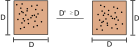
\includegraphics[width=0.7\linewidth]{images/ch_2/low_rank.pdf}
    \caption{Given two boxes in $\mathbb{R}^d$ ($d=2$ or 3), $\mathcal{B}_1$ and $\mathcal{B}_2$, which each enclose a corresponding set of points. The off-diagonal blocks in the matrix $K_{\mathcal{B}_1\mathcal{B}_2}$ and $K_{\mathcal{B}_2\mathcal{B}_1}$ are considered low rank and amenable to compression for the FMM when the distance separating them is at least equal to their diameter.}
    \label{fig:chpt:2:sec:0:rank_decay}
\end{figure}
